\section{Conclusion}

\begin{frame}
	\begin{center}
		\huge Conclusion
	\end{center}
\end{frame}

\begin{frame}
	\frametitle{Conclusion}
	\begin{itemize}
		\item Recent discoveries put our results into question
		\item Results are not verified
		\item Further testing necessary
	\end{itemize}
\end{frame}

\section{Future Work}

\begin{frame}
	\begin{center}
		\huge Future Work
	\end{center}
\end{frame}

\begin{frame}
	\frametitle{Next Semester}
	\begin{itemize}
		\item Rethinking the method
		\item Obtaining a dataset
	\end{itemize}
\end{frame}

\begin{frame}
	\frametitle{Rethinking the Method}
	\begin{itemize}
		\item Reordering of Rank Lists
		\item Ratings as satisfaction measure
		\item Alternative Rank Aggregation
		\item Scaling Matrix Factorization
	\end{itemize}
\end{frame}

\begin{frame}
	\frametitle{Obtaining a Dataset}
	\begin{columns}
		\begin{column}{0.5\textwidth}
			\begin{itemize}
				\item Clickworker
				\begin{itemize}
					\item Crowdsourcing platform with over 800.000 users
					\item Cost as low as 14 Euro cents per user surveyed
				\end{itemize}
			\end{itemize}
			\begin{figure}
				\centering
				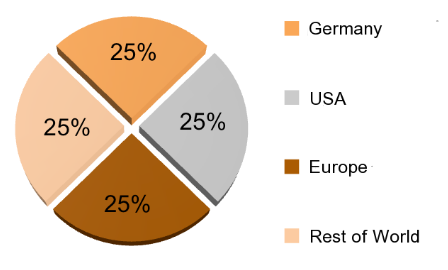
\includegraphics[scale=0.3]{figures/clickworker_users.png}
			\end{figure}
			\footnotetext{https://www.clickworker.com/about-us/clickworker-crowd/}
		\end{column}
		\begin{column}{0.5\textwidth}
			\begin{figure}
				\centering
				\includegraphics[scale=0.5]{figures/crowdsourcing.png}
			\end{figure}
		\end{column}
	\end{columns}
\end{frame}

\begin{frame}
	\frametitle{Clickworker Survey Options}
	\begin{columns}
		\begin{column}{0.5\textwidth}
			\begin{itemize}
				\item Normal survey
			\end{itemize}
			\begin{figure}
				\centering
				\includegraphics[scale=0.4]{figures/Internal_survey_option.png}
			\end{figure}
		\end{column}
		\begin{column}{0.5\textwidth}
			\begin{itemize}
				\item External survey
			\end{itemize}
			\begin{figure}
				\centering
				\includegraphics[scale=0.4]{figures/External_survey_option.png}
			\end{figure}
		\end{column}
	\end{columns}
\end{frame}

\begin{frame}
	\frametitle{Clickworker Survey Tool}
	\begin{columns}
		\begin{column}{1\textwidth}
			\begin{figure}
				\centering
				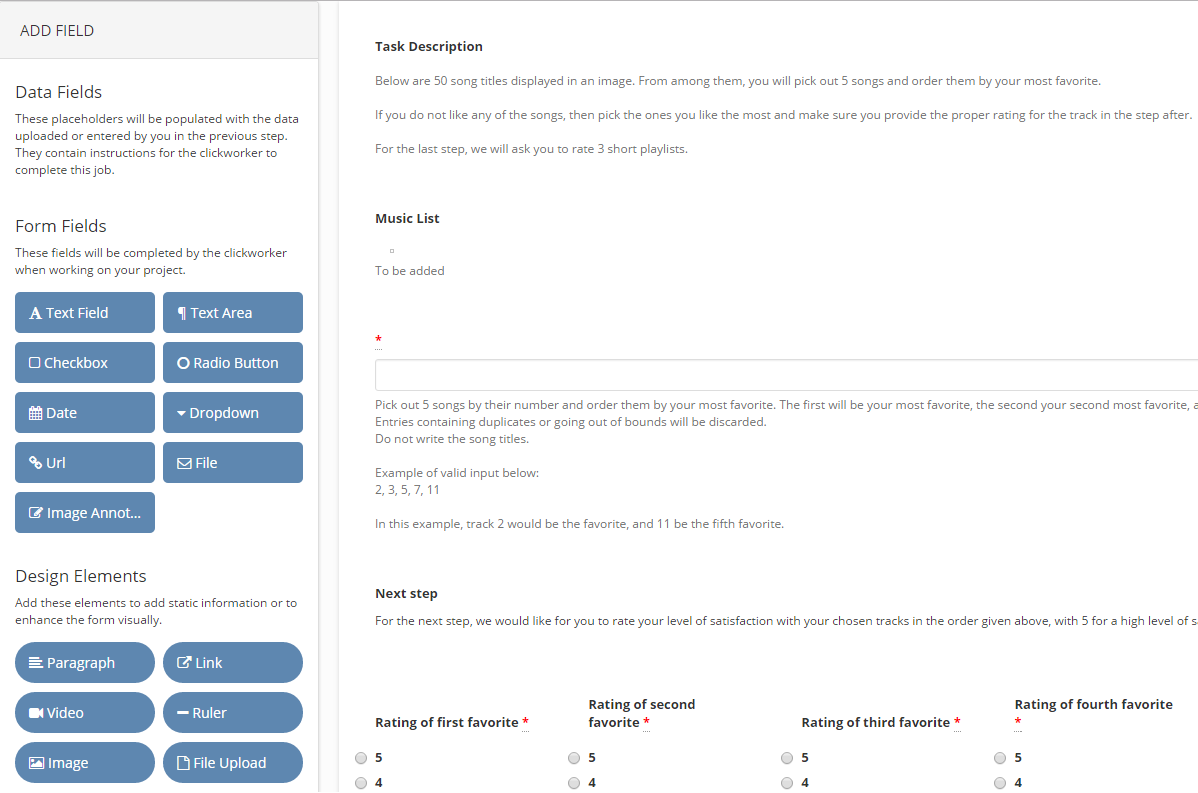
\includegraphics[scale=0.3]{figures/InternalSurvey.png}
			\end{figure}
		\footnotetext{https://marketplace.clickworker.com}
		\end{column}
	\end{columns}
\end{frame}

\begin{frame}
	\frametitle{External Survey}
	\begin{columns}
		\begin{column}{1\textwidth}
			\begin{figure}
				\centering
				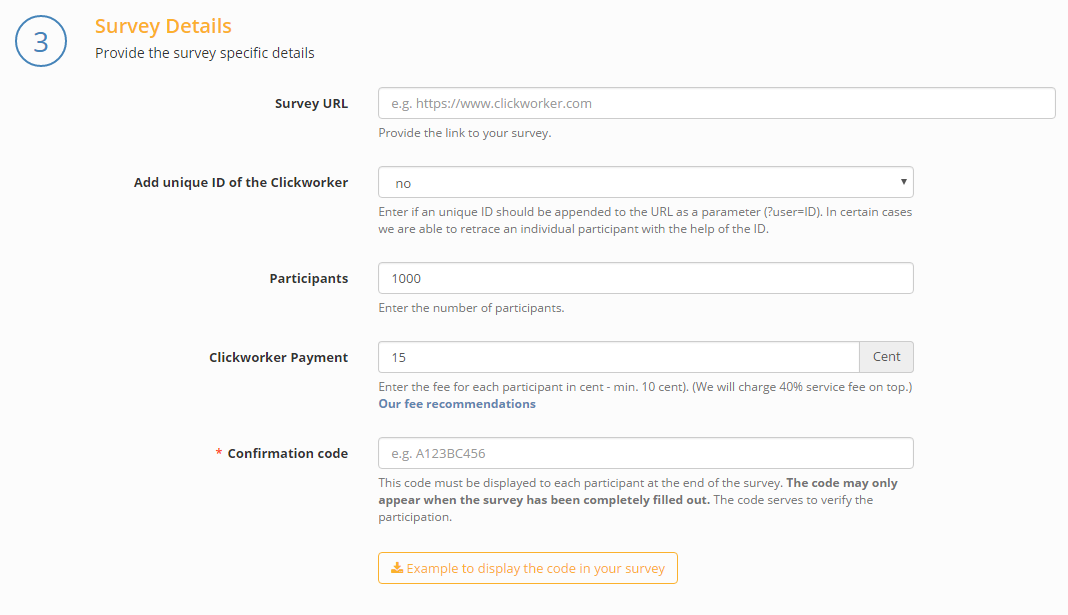
\includegraphics[scale=0.4]{figures/external_survey_details.png}
			\end{figure}
			\footnotetext{https://marketplace.clickworker.com}
		\end{column}
	\end{columns}
	\note{
		Allows us to refer to a URL where we could have a google forms survey
		Google forms is built on top of javascript - allowing us to make the information respond to the user
		Verification code
	}
\end{frame}

\begin{frame}
	\frametitle{Google Forms}
	\begin{columns}
		\begin{column}{0.4\textwidth}
			\begin{itemize}
				\item Built on Javascript
				\item Tailored survey questions
				\item Validation questions
			\end{itemize}
		\end{column}
		\begin{column}{0.6\textwidth}
			\begin{figure}
				\centering
				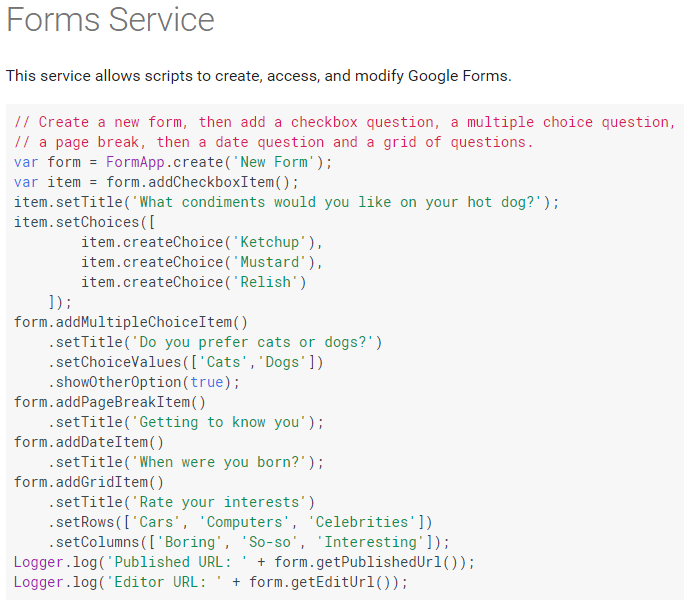
\includegraphics[scale=0.35]{figures/GoogleScript.png}
			\end{figure}
			\footnotetext{https://developers.google.com/apps-script/reference/forms/}
		\end{column}
	\end{columns}
\end{frame}

\begin{frame}
	\frametitle{Internal vs External Survey}
	\begin{columns}
		\begin{column}{0.4\textwidth}
			\begin{itemize}
				\item Internal Survey
				\begin{itemize}
					\item Quick
					\item Simple
					\item Static
					\item Limited return
					\item Bound to Clickworker
				\end{itemize}
			\end{itemize}
		\end{column}
		\begin{column}{0.6\textwidth}
			\begin{itemize}
				\item External Survey
				\begin{itemize}
					\item Time Consuming
					\item Complex
					\item Dynamic
					\item Medium return
					\item Adaptable to most platforms
				\end{itemize}
			\end{itemize}
		\end{column}
	\end{columns}
\end{frame}